\title{CS 613 - Machine Learning}
\author{
        Assignment 2 - Linear Regression\\
        Alex Lapinski\\
        Fall 2016
}
\date{10/20/2016}
\documentclass[12pt]{article}
\usepackage[margin=0.7in]{geometry}
\usepackage{graphicx}
\usepackage{float}
\usepackage{comment}
\usepackage{amsmath}
\graphicspath{{../graphs/}}

\begin{document}
\maketitle

\section{Theory}
\begin{enumerate}
\item Consider the following data:\\
\begin{center}
$
 \begin{bmatrix}
	-2 & 1\\
	-5 & -4\\	
	-3 & 1\\
	0 & 3\\
	-8 & 11\\
	-2 & 5\\
	1 & 0\\
	5 & -1\\
	-1 & -3\\
	6 & 1\\
\end{bmatrix}
$
\end{center}
	\begin{enumerate}
	\item Compute the coefficients for the linear regression using global least squares estimate (LSE) where the second value is the dependent variable (the value to be predicted).  Show your work and remember to add a bias feature and to standardize the features (10pts).\\
	\end{enumerate}
\end{enumerate}


\newpage
\section{Closed Form Linear Regression}\label{linreg}

\begin{enumerate}
\item Final Model: $y=3343.27586207+1036.63016523x_{:,1} - 295.66859639x_{:,2}$
\item Root Mean Squared Error: $653.76012597$
\end{enumerate}

\section{S-Folds Cross-Validation}\label{linreg}

\begin{enumerate}
\item With S = 5 (as required), RMSE = 636.315054765
\item With S = 6 (to test other values), RMSE = 621.823391267
\item With S = 7 (to test other values), RMSE = 640.86061133
\end{enumerate}

\section{Locally-Weighted Linear Regression}
\begin{enumerate}
\item With k = 1 (as required), RMSE = 895.876676714
\item With k = 2 (to test other values), RMSE = 637.726596574
\item With k = 3 (to test other values), RMSE = 616.643575718
\item With k = 4 (to test other values), RMSE = 625.745432869
\end{enumerate}


\newpage
\section{Gradient Descent}

\textbf{Results when $\alpha=0.01$}
\begin{itemize}
\item Final model: $y = 3343.27574946 + 1036.63010327x_{:,1} + -295.66858438x_{:,2}$
\item After 1712 iterations
\item RMSE = 653.760066367
\end{itemize}

\begin{figure}[H]
\begin{center}
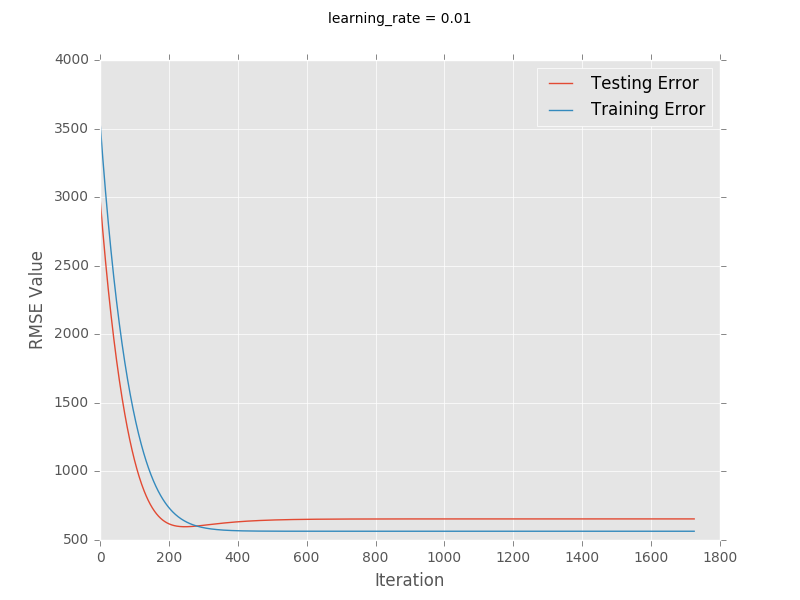
\includegraphics{gradient_descent_errors.png}
\caption{Gradient Descent Progress}
\label{GD}
\end{center}
\end{figure}

\textbf{Results when $\alpha=0.1$}
\begin{itemize}
\item Final model: $y = 3343.27584461 + 1036.63015469x_{:,1} + -295.66859449_{:,2}$
\item After 181 iterations
\item RMSE = 653.760097303
\end{itemize}

\end{document}